\documentclass[tikz, border=5pt]{standalone}

% Semantic GitHub colors for the light theme.
% The Poe task embeds the dark palette from theme-dark.css into each SVG.
\usepackage{tikz}
\usepackage{amsmath, amssymb}
\usetikzlibrary{arrows.meta, calc, positioning, decorations.pathreplacing}

% Text and surfaces.
\definecolor{ghtext}{HTML}{1F2328}
\definecolor{ghmuted}{HTML}{59636E}
\definecolor{ghborder}{HTML}{D0D7DE}
\definecolor{ghpanel}{HTML}{F6F8FA}

% Accent colors and their softer backgrounds.
\definecolor{ghblue}{HTML}{0969DA}
\definecolor{ghbluesoft}{HTML}{DDF4FF}
\definecolor{ghgreen}{HTML}{1A7F37}
\definecolor{ghgreensoft}{HTML}{DAFBE1}
\definecolor{ghpurple}{HTML}{8250DF}
\definecolor{ghpurplesoft}{HTML}{FBEFFF}
\definecolor{ghorange}{HTML}{9A6700}
\definecolor{ghorangesoft}{HTML}{FFF1BA}
\definecolor{ghred}{HTML}{CF222E}
\definecolor{ghredsoft}{HTML}{FFEBE9}

\tikzset{
    >={Stealth[length=2.1mm, width=1.2mm]},
    card/.style={
        fill=ghpanel,
        draw=ghborder,
        rounded corners=2.6mm,
        line width=0.6pt,
    },
    heading/.style={font=\sffamily\small\bfseries, text=ghtext},
    regular/.style={font=\sffamily\small, text=ghtext},
    note/.style={font=\sffamily\footnotesize, text=ghmuted},
    tinylabel/.style={font=\sffamily\scriptsize, text=ghmuted},
    mathlabel/.style={font=\sffamily\small, text=ghtext},
    bluearrow/.style={-Stealth, draw=ghblue, line width=1.5pt},
    purplearrow/.style={-Stealth, draw=ghpurple, line width=1.4pt},
    thin/.style={draw=ghborder, line width=0.7pt},
}


\begin{document}
    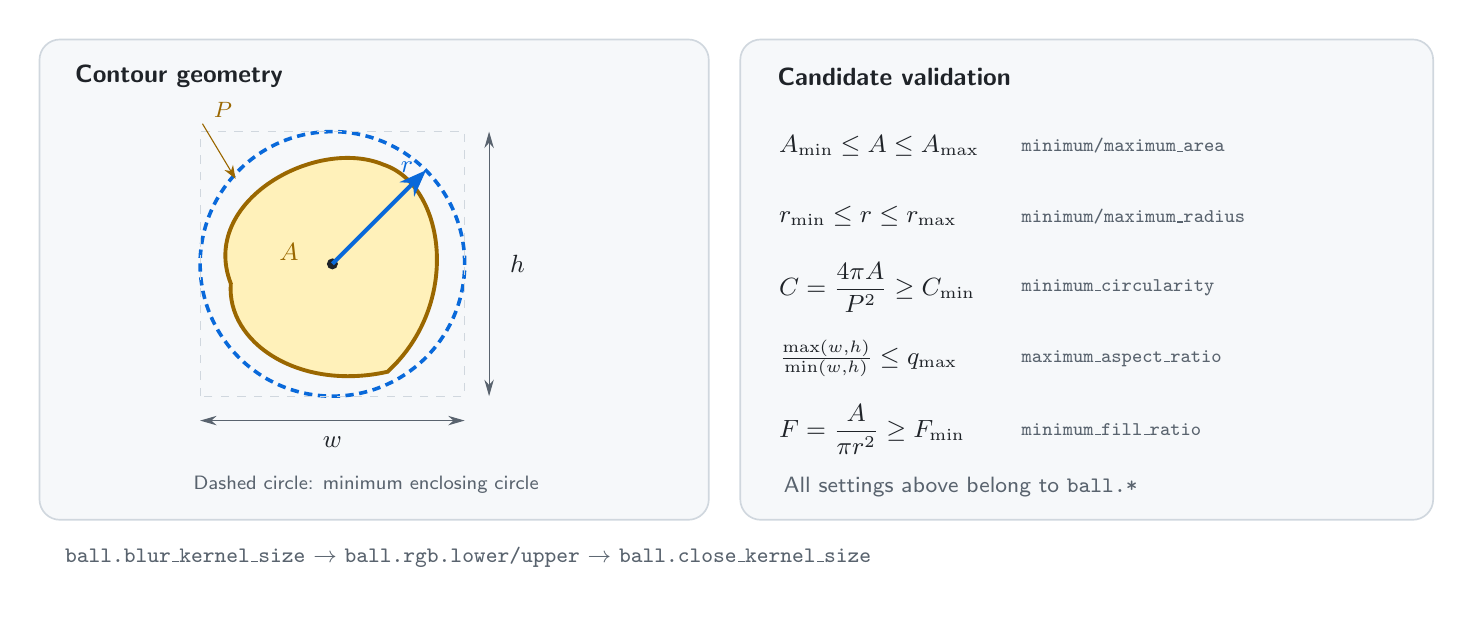
\begin{tikzpicture}[x=1cm, y=1cm]
        \path[use as bounding box] (0, 0) rectangle (18, 7.25);

        % Geometry and constraints panels.
        \draw[card] (0.15, 1) rectangle (8.65, 7.1);
        \draw[card] (9.05, 1) rectangle (17.85, 7.1);

        \node[heading, anchor=west] at (0.48, 6.63) {Contour geometry};
        \node[heading, anchor=west] at (9.4, 6.63) {Candidate validation};

        % Contour, enclosing circle, radius, area, and perimeter.
        \begin{scope}[shift={(3.87, 4.25)}]
            \draw[ghblue, densely dashed, line width=1.3pt]
                (0, 0) circle (1.68);
            \path[fill=ghorangesoft, draw=ghorange, line width=1.4pt]
                (-1.29, -0.25)
                .. controls (-1.7, 0.8) and (-0.2, 1.62) .. (0.65, 1.26)
                .. controls (1.43, 1) and (1.65, -0.5) .. (0.7, -1.37)
                .. controls (-0.42, -1.62) and (-1.35, -1) .. cycle;
            \draw[ghborder, dashed]
                (-1.68, -1.68) rectangle (1.68, 1.68);
            \fill[ghtext] (0, 0) circle (0.07);
            \draw[bluearrow] (0, 0) -- (1.19, 1.19);

            \node[mathlabel, anchor=south east, text=ghblue]
                at (1.15, 1.04) {$r$};
            \node[mathlabel, text=ghorange] at (-0.55, 0.15) {$A$};
            \draw[ghorange, -Stealth] (-1.65, 1.78) -- (-1.23, 1.08);
            \node[note, anchor=west, text=ghorange]
                at (-1.63, 1.96) {$P$};

            \draw[ghmuted, <->] (-1.68, -1.99) -- (1.68, -1.99);
            \node[mathlabel] at (0, -2.26) {$w$};
            \draw[ghmuted, <->] (1.99, -1.68) -- (1.99, 1.68);
            \node[mathlabel] at (2.35, 0) {$h$};
        \end{scope}

        \node[tinylabel] at (4.3, 1.44)
            {Dashed circle: minimum enclosing circle};

        % Filter conditions. All keys belong to ball.* in config.jsonc.
        \node[regular, anchor=west] at (9.42, 5.75)
            {$A_{\min}\leq A\leq A_{\max}$};
        \node[tinylabel, anchor=west] at (12.5, 5.75)
            {\texttt{minimum/maximum\_area}};

        \node[regular, anchor=west] at (9.42, 4.85)
            {$r_{\min}\leq r\leq r_{\max}$};
        \node[tinylabel, anchor=west] at (12.5, 4.85)
            {\texttt{minimum/maximum\_radius}};

        \node[regular, anchor=west] at (9.42, 3.95)
            {$C=\dfrac{4\pi A}{P^2}\geq C_{\min}$};
        \node[tinylabel, anchor=west] at (12.5, 3.95)
            {\texttt{minimum\_circularity}};

        \node[regular, anchor=west] at (9.42, 3.05)
            {$\frac{\max(w,h)}{\min(w,h)}\leq q_{\max}$};
        \node[tinylabel, anchor=west] at (12.5, 3.05)
            {\texttt{maximum\_aspect\_ratio}};

        \node[regular, anchor=west] at (9.42, 2.15)
            {$F=\dfrac{A}{\pi r^2}\geq F_{\min}$};
        \node[tinylabel, anchor=west] at (12.5, 2.15)
            {\texttt{minimum\_fill\_ratio}};

        \node[note, anchor=west] at (9.48, 1.42)
            {All settings above belong to \texttt{ball.*}};

        % Preprocessing pipeline.
        \node[note, anchor=west] at (0.35, 0.53)
            {\texttt{ball.blur\_kernel\_size} $\rightarrow$
             \texttt{ball.rgb.lower/upper} $\rightarrow$
             \texttt{ball.close\_kernel\_size}};
    \end{tikzpicture}
\end{document}
